\documentclass[11pt]{article}
\usepackage[utf8]{inputenc}
\usepackage[T1]{fontenc}
\usepackage{amsmath}
\usepackage{amsfonts}
\usepackage{amssymb}
\usepackage[version=4]{mhchem}
\usepackage{stmaryrd}
\usepackage{graphicx}
\usepackage[export]{adjustbox}
\graphicspath{ {./images/} }

\begin{document}
Activist Investing

Corporate governance describes the processes and people that control the decisions of a corporation. Activist investing is involvement in corporate governance as an alpha-driven investment strategy. The activist investment strategy involves efforts by shareholders to use their rights, such as voting power or the threat of such power, to influence corporate governance to their financial benefit as shareholders. An activist investment strategy often involves (1) identification of corporations whose management is not maximizing shareholder wealth; (2) establishment of investment positions that can benefit from particular changes in corporate governance, such as replacement of existing management; and (3) execution of the corporate governance changes that are perceived to benefit the investment positions that have been established.

\section*{Background on Corporate Governance}
The equity investors in a firm literally establish the corporation and legally own the corporation. But in major corporations, it is impractical for several thousand or million individual shareholders to manage the company on a day-to-day basis. Corporations are therefore set up with a corporate governance process, wherein shareholders elect a board of directors. The board of directors selects and contracts with the executive management team and delegates the management of the company to the executive managers, who are compensated for running the day-to-day business. The top executive managers usually serve as directors of the corporation but with insufficient seats to form a majority.

The firm's executive management team typically provides information to the board regarding the firm's operations and initiates proposals. Although the procedures and levels of consensus vary widely, it is common for the board's decisions to be agreeable with the management team. In other words, the management team and the board of directors tend to work cooperatively. To the extent that the management team is in substantial and irresolvable conflict with the majority of the directors, the management team will be replaced.

The board periodically conducts voting by shareholders for election of new board members and with regard to major proposals. Typically, proposals clearly identify those actions recommended by the board of directors. Shareholders approve the vast majority of board recommendations.

Although shareholders vote for the board of directors and the board selects managers charged with serving the interests of the shareholders, there are typically substantial conflicts between the interests of shareholders and managers. The divergence between the preferences of shareholders and managers is the foundation for most shareholder activism. Shareholder activism refers to efforts by one or more shareholders to influence the decisions of a firm in a direction contrary to the initial recommendations of the firm's senior management. These efforts can include casting votes, introducing shareholder resolutions, and taking legal action. The divergence between the preferences of shareholders and those of managers is a critical issue in understanding shareholder activism and is discussed in detail in a subsequent section.

The terms used to discuss activist investing overlap with terminology used elsewhere in investments and are not used entirely uniformly in discussing shareholder activism. This book defines an activist investment strategy as any investment strategy with the objective of generating superior rates of return through shareholder activism.

One of the most important events of shareholder activism is a shareholder vote. Shareholder votes occur at regular annual meetings and at special shareholder meetings. Shareholders attend meetings to cast their votes, cast direct votes prior to meetings using ballots provided to them by the firm, or complete proxies that allow others to vote on their behalf-either with regard to a specific issue or in general. The outcome of these votes typically depends on the results of a proxy battle. A proxy battle is a fight between the firm's current management and one or more shareholder activists to obtain proxies (i.e., favorable votes) from shareholders. These proxies permit them to vote the shares of the other shareholders in support of their activism. The board of directors can also solicit proxies from shareholders for their support. The proxies help determine the winner of the shareholder vote.

Shareholders can be inundated with multiple copies of the proxy from each side, since each shareholder's ultimate vote is governed by the latest dated or most recently submitted proxy, if any, that the shareholder completed. Proxy battles can be very expensive. Shareholder activists pay for their direct costs of these proxy battles in the hope of financial gains from success. The firm's current board of directors generally uses the corporation's financial resources to wage the battle, which, of course, ultimately belong to the shareholders. Thus, shareholder activists not only pay for their side of the battle but also pay their pro rata share of the other side.

\section*{Five Dimensions of Shareholder Activists}
The players in the arena of shareholder activism differ on several dimensions:

\begin{itemize}
  \item Financial versus social activists: Efforts by shareholder activists can have social objectives or financial objectives. Social objectives include attempts to steer a firm toward behavior deemed by some as more beneficial to society as a whole, such as reduced pollution, better treatment of employees, better treatment of animals, or refusal to manufacture goods such as weapons, alcohol, and tobacco. Financial objectives may vary in some regards, but the underlying motivation is increased shareholder wealth through increased share prices. For the purposes of this chapter, shareholder activist investment strategies refer entirely to shareholder activism driven by financial objectives.
  \item Activists versus pacifists: Activists oppose current management and seek major changes in a firm's leadership or decision-making. Pacifists oppose the proposed activism. Instead, pacifists support current management, the status quo, and any proposed changes outlined by the current management. Activists attempt to intervene in the corporate governance process, whereas pacifists oppose making any changes. Pacifists, however, are not necessarily dormant; they may be aggressive in their opposition to the activists.
  \item Initiators versus followers: Some shareholders initiate activism, whereas others actively follow the activists. Activists can be followed through stories in the media or through required regulatory filings, such as 13D forms. Initiators of activism search for suitable targets, develop activist plans, establish positions, and implement the plans. Importantly, initiators pay for the direct expenses of activism. Active followers support the plans of the initiators and establish positions in the firms being targeted by activists.
  \item Friendly versus hostile activists: Activism is executed with different degrees of confrontation with management. Hostile activists tend to threaten managers with adverse consequences, whereas friendly activists tend to work with managers to develop mutually beneficial outcomes. Whereas some activists prefer to\\
engage corporate management behind closed doors, others conduct very public campaigns, with their demands distributed through the media. When conversations are public, other large shareholders-both hedge funds and pension funds-may get involved in the conversation or voting process.
  \item Active activists versus passive activists: This dimension refers to the motive for investing. Active activists establish positions for the purpose of activism. Passive activists participate in activism when they happen to hold positions in firms that become targets of activism. It is also possible but less likely for passive activists to be initiators rather than followers. A passive activist can be an initiator by first establishing a position for purposes other than activism but then deciding to initiate activism, perhaps due to frustration with current management.
\end{itemize}

\section*{Shareholder Activists' Strategies}
The key players in successful financial activism are active initiators, active followers, and passive followers. The role of active initiators is obvious, since they serve as the catalysts for the actions and typically bear the potentially large direct costs involved. But active initiators rarely have sufficient voting power to implement change unless others join in. Activists need to be careful about hunting in packs, as securities laws may be violated if activists work together without the proper regulatory disclosures. In order to avoid the appearance of working in groups, Orol encourages activists to choose separate law firms and to avoid emailing one another. ${ }^{1}$ Ronald D. Orol (2008), Extreme Value Hedging: How Activist Hedge Fund Managers Are Taking on the World (Hoboken, NJ: John Wiley \& Sons).

Passive activists, those who have positions in firms where an activist is leading the efforts, may be viewed as free riders. A free rider is a person or entity that allows others to pay initial costs and then benefits from those expenditures. An example of a free rider is a citizen who stands by while a subgroup pays for an improvement, such as the beautification of a park, and then enjoys the enhancement. Shareholder activism can have large direct costs, including legal costs and the costs of proxy contests. Active followers search public records and other sources of information to identify firms that are most likely to be profitable targets of shareholder activism. For example, active followers can directly or indirectly learn of potential activism targets from observing that known shareholder activists are acquiring positions in particular firms. Regulators often require information on large holdings by market participants. Active followers have a symbiotic relationship with active initiators. Although they act as free riders to the active initiators who pay the direct costs of activism, active followers typically help the initiators by voting in support of the activism, which serves to increase the influence of the initiators without their having a larger investment in the target firm.

Most investors are passive in the context of this analysis; that is, these investors, like those in mutual funds, established positions in the equity of public companies for reasons other than anticipation of activism. Passive followers, or the lack thereof, often make or break shareholder activism. Passive followers are a subgroup of the passive investors who happen to be holding stock in a firm that becomes the target of activist initiators. These existing shareholders who retain their shares must ultimately decide whether they will support the activist proposals as passive followers or vote against the proposals as pacifists. They can become the object of intense battles between activist initiators and agents of the firm's management, receiving mailings, overnight correspondence, phone calls, and even personal contacts from both sides soliciting their support.

The key players in unsuccessful financial activism are pacifists. These shareholders do not establish equity positions in the target firm for the purposes of supporting or opposing activism. They are brought into the fray from holding previously established positions in firms that became the targets of activism. They opt to support current management due to confidence in the management or a belief that the activists would be harmful. In addition, some shareholder pacifism results from concerns that support for the activists might damage their business relationships with current management and other entities that oppose the activism. Shareholder votes are not secret ballots; thus, corporate management generally has direct knowledge of which shareholders vote to support their position and which shareholders oppose them.

\section*{Why Managers Are Not Viewed as Maximizing Shareholder Wealth}
As their name implies, activist investors believe that value can be unlocked within a public company through active engagement with the executive management of the corporation or its board of directors. A common question is why the executive management of the company does not undertake the necessary changes to unlock the intrinsic value of the company without pressure from activists. The fundamental reason is the existence of conflicts of interest between managers and shareholders. Simply put, managerial goals can differ from shareholder goals.

Agency theory studies the relationship between principals and agents. A principal-agent relationship is any relationship in which one person or group, the principal(s), hires another person or group, the agent(s), to perform decision-making tasks. The principals enter this relationship with the objective of having their utility maximized, while the agents seek to maximize their own utility. Preferences and goals generally differ among all people and all groups of people. Therefore, conflicts of interest typically exist within all organizations and among all groups within those organizations.

Shareholders are the principals and the executive management team members are their agents. It is generally reasonable to assume that as principals, the shareholders wish to have the managers pursue shareholder wealth maximization (share price plus dividends), whereas the managers wish to pursue their goals, including salary maximization, bonus maximization, prestige, career opportunities, job security, job satisfaction, and perhaps improved leisure time and other aspects of their lives. To the extent that shareholder wealth maximization is inconsistent with the goals and preferences of managers, there will be conflicts of interest.

Agency theory focuses on optimal contracting in the presence of conflicts of interest-specifically on the process of designing managerial compensation schemes that maximize shareholder wealth. An agent compensation scheme is all agreements and procedures specifying payments to an agent for services, or any other treatment of an agent with regard to employment. A perfect compensation scheme would be costless to implement and would maximize shareholder wealth by resolving all conflicts of interest between shareholders and managers at minimal cost.

In practice, however, perfect compensation schemes do not exist, resulting in agency costs. In a nutshell, agency costs are any costs, explicit (e.g., monitoring and auditing costs) or implicit (e.g., excessive corporate perks), resulting from inherent conflicts of interest between shareholders as principals and managers as agents. These agency costs have two sources: (1) the costs of aligning the interests of shareholders and managers when those interests can be cost-effectively aligned, and (2) the costs to the shareholders of unresolved conflicts of interest between shareholders and managers. Regarding the latter source, not all conflicts of interest can be cost-effectively resolved; therefore, in an optimal compensation scheme, agents will generally not always act in the best interests of the principals. Simply put, in some cases, it is cheaper for shareholders to accept managerial actions that conflict with their best interests than to try to bring managers' interests into perfect alignment with their own interests.

\section*{Consequences of Shareholder and Manager Misalignment}
The misalignment between shareholders' and managers' interests stemming from unresolved conflicts of interest often results in potentially major and inefficient consequences, including the following:

\begin{itemize}
  \item Managers receiving excessive compensation from running the corporation for their own personal entitlement at disproportionately large costs to shareholders
  \item Managers being overly risk averse in their decision-making for fear of being associated with large failures and possibly losing job security
  \item Managers making decisions (with disproportionately large costs to shareholders) based on the comfort they obtain from protecting their jobs and existing pay packages
  \item Managers imposing risk preferences in corporate decision-making based on their disproportionate participation in the upside of the company's fortunes and their limited downside exposure
  \item Managerial preferences to avoid hard work or reject optimal change, such as updating the business plan or model of the company, which disproportionately harm shareholder wealth
  \item Managerial preferences to avoid sharp conflicts, such as challenging unions, demoting employees, firing employees, or closing divisions
\end{itemize}

In each case, there is nothing suboptimal about a manager receiving generous compensation or avoiding a personally undesirable outcome as long as there is not a net unnecessary cost to shareholders. To illustrate, it may be economically efficient for a firm to offer free parking to a manager in exchange for reduced taxable salary if there is a net benefit to that combination that increases shareholder wealth. Further, it may serve the best interests of shareholders to offer first-class airfare, or even corporate jet travel, to managers if such actions ultimately create value and a net benefit to shareholders, perhaps through employee satisfaction and resulting improved performance. The examples were designed to emphasize conflicts of interest that tend to be inefficient when managers receive benefits or engage in behavior that has high costs without offsetting benefits to shareholders. Shareholders are not averse to paying generous financial and other benefits to managers who are thereby incentivized to offer services that provide net benefits to shareholders. Rather, shareholders are concerned with compensation to managers or behavior by managers with costs deemed excessive or disproportionate relative to the benefits these managers generate.

In large public corporations, the practical ability of shareholders to understand, monitor, and correct conflicts of interest with managers may be very limited. As a result, conflicts of interest may emerge and grow that are inefficient and, in aggregate, may become highly costly to shareholders. As a result of these conflicts based on managerial preferences dominating shareholder interests, a public company's stock price may trade substantially below its intrinsic value. Therein lies the source of untapped value that shareholder activist strategies pursue.

\section*{Corporate Governance Battles}
Rather than waiting for untapped value, or alpha, to be exploited through external events, activists attempt to accelerate the realization of the alpha by seeking to expedite change to the operations of a corporation. The intense engagement required to be an active initiator means that activists must typically hold very concentrated portfolios of 5 to 15 equity positions in publicly traded corporations. These positions are long, are large, and usually represent $1 \%$ to $10 \%$ of the outstanding stock of the company. There is a considerable amount of systematic and idiosyncratic risk embedded in the resulting portfolios. Although the fee structures and liquidity risks clearly categorize activist fund managers as hedge fund managers, some investors may view investments in activist funds to be sufficiently similar to traditional long-only equity investments that they include the activist fund holdings in the computation of their allocation to equity.

Activist hedge fund positions in target firms can be kept secret as long as the activist owns less than 5\% of the target firm. In the United States, Form 13D is required to be filed with the Securities and Exchange Commission (SEC) within 10 days, publicizing an activist's stake in a firm once the activist owns more than $5 \%$ of the firm and has a strategic plan for the firm. Many activists will acquire a $4.9 \%$ stake in the firm, just below the threshold for filing a Form 13D, to keep their holdings secret and to allow time for conversations with the firm to progress. A toehold is a stake in a potential merger target that is accumulated by a potential acquirer prior to the news of the merger attempt becoming widely known.

In addition to Form 13D, several other forms may be required to provide investors with additional information regarding potential mergers. In the United States, Form $13 \mathrm{G}$ is required of passive shareholders who buy a $5 \%$ stake in a firm, but this filing may be delayed until 45 days after year-end. Form $13 \mathrm{~F}$ is a required quarterly filing of all long positions by all US asset managers with over $\$ 100$ million in assets under management, including hedge funds and mutual funds, among other investors. These forms must list all long positions; however, disclosure of short positions is not required.

Many investors regularly track these filings, some taking positions in the holdings of famous or profitable activists and other hedge fund managers. Brav et al. show that companies listed as holdings of activists on Form 13D have a one-month excess return of 7\% during the month of the 13D disclosure while earning returns similar to the market in the following year. ${ }^{2}$ Alon Brav, Wie Jiang, Frank Partnoy, and Randall Thomas (August 2008), Hedge Fund Activism, Corporate Governance and Firm Performance, Journal of Finance 63 (no. 4): 1730. This return is not consistent across activist objectives, as activist goals of mergers earn $10 \%$ returns and exploring strategic alternatives earns $5.9 \%$ returns, whereas corporate governance issues have no statistically significant excess returns.

Well-respected activists may have a strong following or wolf pack of other hedge funds (active followers). A wolf pack is a group of investors who may take similar positions to benefit from an activists' engagement with corporate management. This wolf pack investment team can magnify the activists' influence, as the combined positions of similarly minded investors serve to make the target firm's management more responsive to the activists' agenda.

Activists typically publicize a single issue that is believed to add substantial value to the shares of the target firm. Activist agendas have targeted a wide variety of corporate governance issues, including executive compensation, composition of the board of directors, potential mergers or divestitures, and capital structure issues such as cash positions that are too large and debt loads or dividends that are too low.

Activist investors usually demand a meeting with the target company's board of directors or senior management to discuss and publicize the desired change in corporate governance. In addition, activist investors may attempt to work with management to implement their preferred business plan. This manner of investing is friendly and is also called corporate engagement, as activist investors pursue a direct dialogue with management and the board of directors. Alternatively, or subsequently, activist investors may resort to hostile actions, such as attempts to remove senior management who are perceived as unresponsive or ineffective.

Although activists have been accused of thinking only about short-term stock price movements, the management of the target firm may be more inclined to agree to the activists' agenda when it is perceived to be likely to lead to longer-term creation of value for the corporation. Activists can have quite lengthy holding periods, frequently owning a stock for one to three years before the value has been unlocked.

The success of investors such as CalPERS and Hermes has encouraged other investors to engage corporation management to reap the rewards of better corporate governance. Using a large hand-collected data set from 2001 to 2006, Brav et al. ${ }^{3}$ Ibid, 1729. find that hedge fund activists succeed in at least part of their agenda at\\
two-thirds of the target firms. Target firms in the United States experience increases in operating performance, payout, and CEO turnover after activism from hedge funds.

It can be more difficult for activist investors to earn a large number of board seats when the terms of the board members are staggered. Staggered board seats exist when instead of having all members of a board elected at a single point in time, portions of the board are elected at regular intervals. For example, if one-third of the board seats are elected each year, it would take at least two years to elect a majority of the board. Corporations are more vulnerable when the entire board is up for election in a single year, because activists can more quickly take control of the board.

\section*{Activist Agenda 1: CEOs, Compensation, and Boards of Directors}
Good corporate governance efficiently resolves those conflicts of interest that are worth resolving. Interlocking boards occur when board members from multiple firms-especially managers-simultaneously serve on each other's boards and may lead to a reduced responsiveness to the interests of shareholders. Interlocking boards and exorbitant CEO compensation are typical conflicts of interest that merit resolution and are near the top of the activist agenda. Conflicts of interest and resulting agency costs can become particularly inefficient when a CEO effectively controls the board of directors in one of two forms. First, the CEO might also be the chairman of the board of directors. In such a position, the CEO-chairman controls both the company's operations and the board of directors, with limited checks and balances. Second, the board of directors can become too comfortable or friendly with the CEO. This can lead to excessive pay packages for the CEO.

An unfortunate example of the latter situation is UnitedHealth Group of Minnesota. For years, UnitedHealth Group's board of directors lavished compensation on William McGuire, the company's CEO and founder. However, more egregiously, the board granted McGuire stock options that were backdated to a point in time when the stock price of the company was lower. The result was that McGuire received a stock option payout in 2006 of $\$ 1.6$ billion, the largest payout for a US corporate CEO at that time. Outrage by activist investors led to a class action lawsuit filed by CalPERS in 2006, which was joined by several other state pension funds. The class action lawsuit was filed against UnitedHealth, 20 executives, and the board of directors, and was quickly followed by an SEC enforcement against McGuire. The result was a settlement reached by the company to return to share owners approximately $\$ 900$ million from backdated stock option grants. Of this amount, $\$ 300$ million came from current executives of UnitedHealth, who agreed to forfeit amounts previously paid. McGuire personally agreed to return more than $\$ 600$ million of his backdated stock option gains. In addition, the SEC fined McGuire $\$ 7$ million and barred him from being a director of a public company for 10 years. McGuire also lost his job at UnitedHealth.

Although it can be appropriate for CEOs to earn large salaries and bonuses, activists believe that total compensation should be incentive based and appropriate relative to the value generated by the management team. For very large corporations, the direct cost of generous compensation schemes is often minor when viewed as a percentage of the firm's equity or income. The concerns with high compensation in very large firms are often more a matter of other issues and can include information signaling and agency costs. Information signaling is the intentional or unintentional conveying of information through actions.

What sort of information signals can large compensation packages to top managers send to the firm's other employees, lenders, and customers? Does a huge managerial compensation package encourage the firm's stakeholders to negotiate more aggressively with the firm or to be less cooperative?

Large non-incentive-based compensation schemes can exacerbate agency conflicts and costs. Managers who are generously paid without serving shareholder interests may focus their energies on serving the stakeholders and the corporate cultures that sustain their pay. The costs to shareholders of ineffective management, from their perspective, may greatly exceed the direct costs of compensation.

\section*{Activist Agenda 2: Capital Structure and Dividend Policy Issues}
Another popular agenda among activists is to request a change in the capital structure or dividend policy of the firm. As a profitable firm accumulates cash, managers have an incentive to reinvest the cash inside the firm so that the firm grows in size and profitability, and presumably the compensation and prestige of the manager will similarly grow. Investors want the firm to exploit those opportunities for which the firm has a comparative advantage through managerial expertise or other capabilities. However, due to unresolved conflicts of interest, managers may have an incentive to invest in opportunities even if they do not exploit the firm's advantages and do not maximize shareholder wealth. Perhaps some investments diversify the firm's assets and thereby provide job security. Improperly incentivized managers may intentionally or inadvertently advocate reinvestment of earnings into projects that are not in the best interests of the shareholders.

Shareholders may believe that it is better to use the cash to pay dividends or execute stock buybacks or share repurchases rather than to reinvest the cash in new businesses through retained earnings. Both dividends and stock buybacks return cash to shareholders. In theory, both can generate equivalent outcomes, since they both reduce the firm's cash and the total market value of the firm's equity. In practice, tax laws often favor share repurchases because personal income taxes on capital gains are usually lower than taxes on dividends. Activists frequently call for increases in dividends or stock buybacks, believing that the cash can be better deployed in the hands of the shareholders. There is an additional benefit of share buybacks in that earnings growth can accelerate. Given that Earnings per Share = Net Income/Shares Outstanding, a decrease in shares outstanding increases earnings per share even when net income is unchanged.

Consider the case of Microsoft, which came under attack after amassing cash of more than $\$ 56$ billion while not paying shareholder dividends. Shareholders were benefiting from the software business, a business that is extremely profitable but usually not capital intensive. Shareholders feared that Microsoft's management would use the cash to expand into unrelated capital-intensive businesses, such as video game consoles and cable television boxes. Microsoft initiated its dividend in 2003 , shortly after US tax laws changed to reduce the tax on dividend income. In 2005, Microsoft paid a one-time dividend of $\$ 32$ billion, announced a stock buyback of $\$ 30$ billion, and doubled the amount of the quarterly dividend. Would retention of the cash have allowed Microsoft to exploit valuable new opportunities, or did the distribution of the cash allow shareholders to deploy the capital more effectively? To the extent that large unresolved conflicts of interest and resulting agency costs exist between shareholders and managers, shareholders have an incentive to serve as activists and intervene to assure the efficient deployment of excess cash.

Activists may also criticize firms for not having enough debt on the balance sheet. In some cases, it is argued that the after-tax cost of debt capital can be below that of the risk-adjusted cost of equity capital, due, for instance, to the tax deductibility of interest expense from corporate taxable income. However, higher leverage increases the risk of the firm's equity and generally increases the probability of the firm experiencing financial distress or bankruptcy. The reason is that, unlike equity financing, debt financing obligates the firm to make mandatory principal and interest payments, which may push the firm into bankruptcy.

Interestingly, once debt has been issued, a firm that is struggling may find that risk-taking that causes higher probabilities of financial distress can increase shareholder wealth. Equity in a corporation can behave like a call option on the firm's assets. Option theory demonstrates that increased volatility in an option's underlying assets increases the value of a call option. Therefore, shareholders may benefit from high levels of risk-taking. Simply put, shareholders can receive full upside benefits from gains while enjoying limited downside exposure to losses because of their ability to declare bankruptcy and leave further losses to be borne by\\
debt holders. Of course, this risk-taking can be limited by other constraints, since a firm with increasing levels of distress may find it difficult to continue attracting the efforts and resources of employees and suppliers.

Managers are very likely to have different preferences than shareholders with regard to risk-taking, meaning there is a conflict of interest. Managers would typically be expected to prefer lower probabilities of corporate financial distress so that their compensation packages and careers are protected. The result can be that managers underutilize debt, leaving wealth-increasing opportunities unexploited. Corporate leverage can also provide benefits to shareholders by disciplining a firm's management to deploy the capital wisely and oversee the firm more closely. The managers of a highly leveraged firm may become more disciplined in their investments and other decisions in order to protect their salaries and careers, since they are aware of the need to meet required debt payments. Conversely, managers of firms with limited leverage and with excess cash obtained through retained earnings may be less disciplined, may have greater conflicts of interest with shareholders, and may subject the firm to greater losses due to agency costs. Accordingly, companies that are underleveraged can be targets of shareholder activism or targets for acquisition as the market attempts to correct the inefficiency.

\section*{Activist Agenda 3: Mergers or Divestitures}
Some mergers and related corporate activity are not driven by shareholder activism but are often related to asset-driven motivations, such as operational efficiencies, conglomeration, integration, and reduction in competition. Merger activity driven by shareholder activism is better understood through viewing such corporate reorganizations as battles for control of assets and analyzing those battles with respect to the interests of managers and shareholders.

Activists are constantly searching to understand business models and the valuations of corporations and their subsidiaries. When an activist finds a portion of a large corporation that is not maximizing shareholder wealth, the activist encourages the corporation to sell or spin off the shares of the business. This situation is especially likely in a conglomerate, in which one firm manages a wide variety of businesses, or in a large firm that has faster-growing, smaller divisions.

A spin-off occurs when a publicly traded firm splits into two publicly traded firms, with shareholders in the original firm becoming shareholders in both firms. For example, a shareholder who owns 300 shares of Company A before a spin-off may own 300 shares of Company A and 100 shares of Company B after the spin-off if each three shares of Company A spun out one share of Company B. A split-off occurs when investors have a choice to own Company A or B, as they are required to exchange their shares in the parent firm if they would like to own shares in the newly created firm.

Consider the case of McDonald's (MCD), which owned a fast-growing business named Chipotle Mexican Grill. McDonald's was encouraged by activists to split the two firms in the belief that the value of the two businesses as independent firms would be higher than the value of the two combined. McDonald's split off Chipotle Mexican Grill (eventually trading as CMG) by performing an initial public offering (IPO) of a small portion of CMG shares and distributing the remaining shares to those MCD shareholders who chose to exchange their shares. The split-off appeared highly successful for investors in both firms, as MCD shares doubled and CMG shares increased by more than $300 \%$ in the first five years after the split-off, while the US stock market was relatively unchanged.

The Chipotle investment was profitable for McDonald's, which purchased 90\% of the young burrito chain for $\$ 360$ million in a series of transactions beginning in 1998. In 2006, the IPO and split-off of CMG earned McDonald's $\$ 1.5$ billion in proceeds. By 2014, it was clear why the split-off occurred, as McDonald's is a large, slowgrowing firm with a market capitalization of $\$ 92.5$ billion and a forward price-to-earnings ratio of 17 . Chipotle had grown quickly to a market capitalization of $\$ 21$ billion and a forward price-to-earnings ratio of 50. While the share price of McDonald's increased by $300 \%$ from 2006 to 2014, Chipotle dramatically outperformed by increasing by $1,200 \%$ over the same period. It is not clear if the value of the CMG business would have increased at such a high rate if it had continued to be housed within the larger MCD holding company.

Another popular activist agenda is to separate hard assets from intellectual property. One example is the trend to separate retail firms from their real estate holdings. In the United States, Pershing Square proposed to separate Target Stores into two companies, one to hold the retail operations and another to restructure the real estate holdings into a REIT (real estate investment trust).

Several explanations can be set forth as to why such corporate reorganizations could increase shareholder wealth. For example, an agency theory-based explanation would be that agency costs are reduced. In both cases, by separating the assets, each resulting management team could manage with better focus. Other explanations are based on capital market inefficiencies or imperfections. For example, some may argue that separation of the ownership of the two units allows different clienteles of shareholders to invest in the business they prefer rather than being allowed to invest only in the combined businesses. Similarly, some may argue that earnings are priced inefficiently in financial markets, such that higher price-to-earnings ratios are applied to the separated earnings streams than to the combined earnings stream.

\section*{Key Observations Regarding Historical Returns of Activist Funds}
Monthly returns to activist funds are observed from January of 2005 to December of 2021 for a total of 204 observations. Statistical Summary of Returns provides univariate return statistics and the partial autocorrelations of returns in the top panel, and a histogram of returns in the bottom panel.

\begin{center}
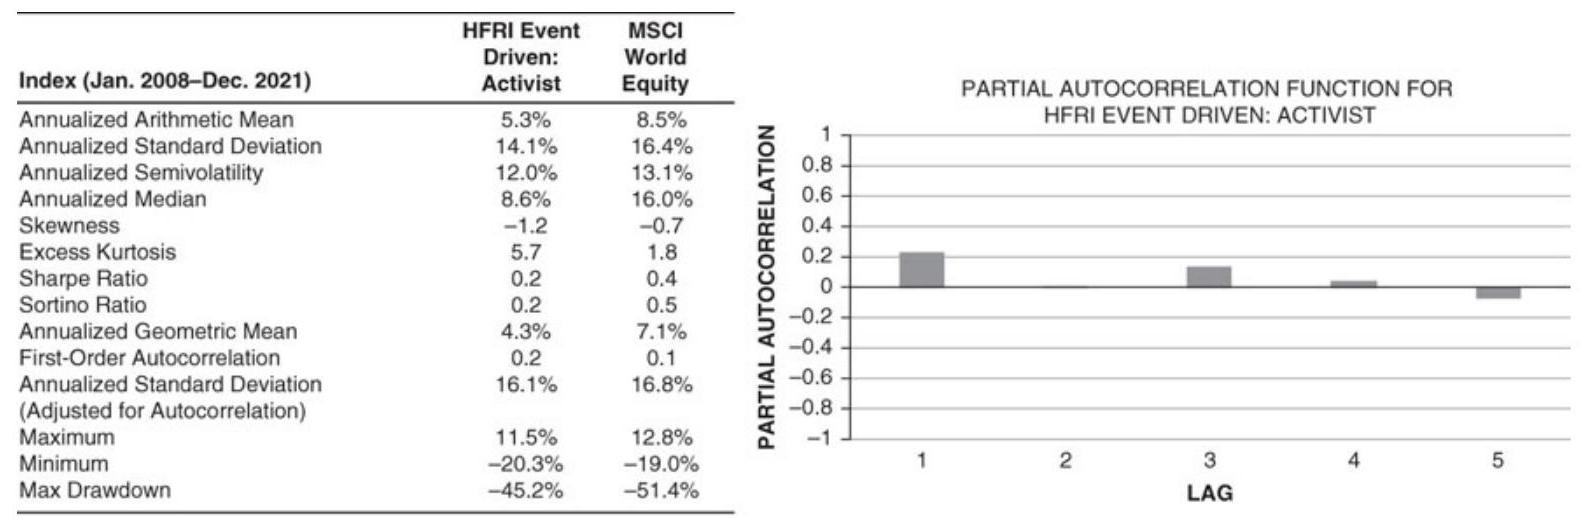
\includegraphics[max width=\textwidth]{2024_04_09_7a731eb4be7055a19322g-7(1)}
\end{center}

Histogram of HFRI Event Driven: Activist Returns (Monthly) Jan. 2008-Dec. 2021

\begin{center}
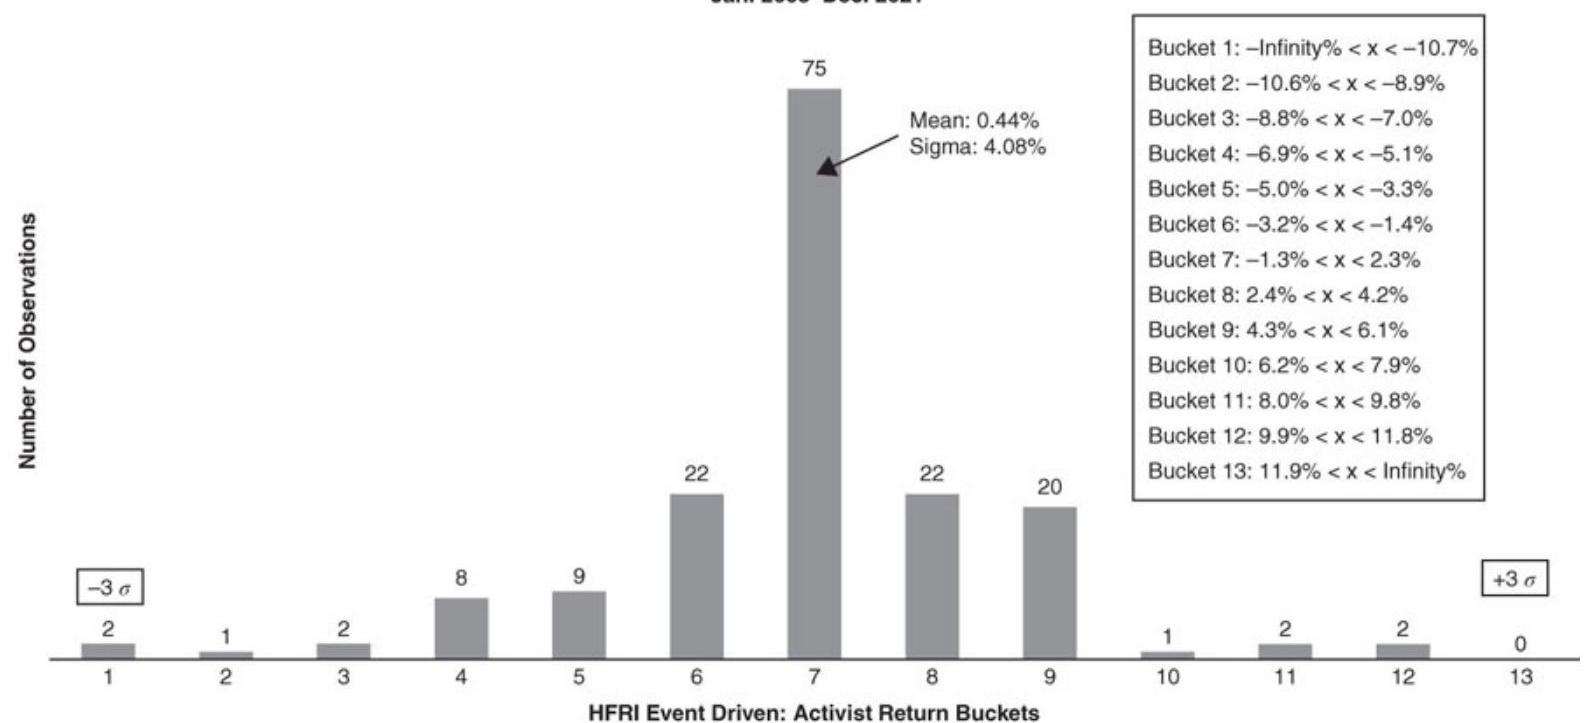
\includegraphics[max width=\textwidth]{2024_04_09_7a731eb4be7055a19322g-7}
\end{center}

\section*{Statistical Summary of Returns}
Key observations on the returns to activist funds that are consistent with economic reasoning are an essential component of knowledge and include the following:

\begin{enumerate}
  \item The volatility, skew, excess kurtosis, and Sharpe ratio are comparable to world equity indices.

  \item Activist hedge funds exhibited lower maximum drawdowns than that of world equities.

  \item Activist returns exhibited positive first- and third-order autocorrelation.

\end{enumerate}

\end{document}